\documentclass[a4paper,12pt]{article}

% ─── Кодировка и язык ───
\usepackage[utf8]{inputenc}
\usepackage[T2A]{fontenc}
\usepackage[russian]{babel}

% ─── Поля ───
\usepackage[left=2.5cm, right=1.5cm, top=2cm, bottom=2cm]{geometry}

% ─── Пакеты ───
\usepackage{graphicx}
\usepackage{booktabs}
\usepackage{longtable}
\usepackage{hyperref}
\usepackage{listings}
\usepackage{xcolor}
\usepackage{caption}
\usepackage{enumitem}
\usepackage{float}
\usepackage{tabularx}
\usepackage{amsmath}
\usepackage{amssymb}

\lstset{
  basicstyle=\ttfamily\small,
  backgroundcolor=\color{gray!10},
  frame=single,
  breaklines=true,
  showstringspaces=false,
}

\hypersetup{
  colorlinks=true,
  linkcolor=blue!60!black,
  urlcolor=blue!70!black,
  citecolor=green!50!black
}

\usepackage{setspace}
\onehalfspacing

\begin{document}

% ═══════════════════════════════════════════
% ТИТУЛЬНЫЙ ЛИСТ
% ═══════════════════════════════════════════

\begin{titlepage}
\begin{center}

\textbf{РОССИЙСКИЙ УНИВЕРСИТЕТ ДРУЖБЫ НАРОДОВ\\ИМЕНИ ПАТРИСА ЛУМУМБЫ}\\[0.3cm]
\textbf{Факультет физико-математических и естественных наук}\\[0.3cm]
Направление подготовки: 09.03.03 <<Прикладная информатика>>\\[2cm]

{\Large \textbf{ЗАДАНИЕ 7}}\\[0.5cm]
{\large \textbf{Результаты вычислительного эксперимента}}\\[1cm]

{\large Тема НИР:}\\[0.3cm]
{\large <<Анализ тональности сообщений пользователей социальных сетей\\
и оценка их влияния на динамику цен криптовалют>>}\\[2cm]

\begin{tabular}{ll}
\textbf{Студент:} & Мугари Абдеррахим \\
\textbf{Группа:} & НФИбд-01-22 \\
\textbf{Науч. рук.:} & доц., к.т.н. Молодченков А.И. \\
\textbf{Трек:} & П (прикладной) \\
\end{tabular}

\vfill
Москва, 2026

\end{center}
\end{titlepage}

\tableofcontents
\newpage

% ═══════════════════════════════════════════
% 1. ПЛАН ЭКСПЕРИМЕНТА
% ═══════════════════════════════════════════

\section{План вычислительного эксперимента}

\subsection{Цель эксперимента}

Оценить наличие и силу статистической взаимосвязи между агрегированными показателями
тональности Twitter-сообщений о Bitcoin и дневной динамикой цен BTC/USD.

\subsection{Гипотезы}

\begin{enumerate}
  \item[$H_1$:] Существует статистически значимая корреляция между дневным средним
        показателем тональности (VADER compound) и дневной доходностью BTC.
  \item[$H_2$:] Тональность сообщений предшествует изменениям цены (предсказательная сила),
        что может быть выявлено тестом Грейнджер-каузальности.
  \item[$H_3$:] Лексиконный метод (VADER) и трансформерная модель (FinBERT)
        дают существенно различающиеся оценки тональности для криптовалютных текстов.
\end{enumerate}

\subsection{Данные}

\begin{table}[H]
\centering
\caption{Параметры датасета}
\label{tab:dataset}
\begin{tabular}{|l|c|}
\hline
\textbf{Параметр} & \textbf{Значение} \\
\hline
Источник & Twitter/X API \\
\hline
Тематика & Bitcoin (BTC) \\
\hline
Период сбора & 26 июля -- 30 августа 2022 г. \\
\hline
Общее число твитов & 664\,918 \\
\hline
Язык & Английский (фильтр \texttt{lang=en}) \\
\hline
Подвыборка для эксперимента & 50\,000 (random, seed=42) \\
\hline
Число уникальных дней & 36 \\
\hline
Источник цен & CoinGecko API (fallback: встроенные данные) \\
\hline
\end{tabular}
\end{table}

\subsection{Методология}

Эксперимент состоит из следующих этапов:

\begin{enumerate}
  \item \textbf{Предобработка:} очистка текста (удаление URL, упоминаний, RT),
        токенизация (NLTK), удаление стоп-слов.
  \item \textbf{Анализ тональности:}
    \begin{itemize}
      \item VADER: оригинальный текст $\rightarrow$ compound score $\in [-1, 1]$.
      \item FinBERT: очищенный текст $\rightarrow$ label $\in \{$positive, neutral, negative$\}$.
    \end{itemize}
  \item \textbf{Агрегация:} ежедневное среднее compound, доля позитивных/негативных,
        стандартное отклонение, число твитов.
  \item \textbf{Ценовые данные:} дневные цены BTC/USD, дневная доходность:
    \begin{equation}
      r_t = \frac{P_t - P_{t-1}}{P_{t-1}}
    \end{equation}
  \item \textbf{Корреляционный анализ:}
    \begin{itemize}
      \item Корреляции Пирсона и Спирмена при лагах $k = 0, 1, \ldots, 7$ дней.
      \item Тест Грейнджер-каузальности: $H_0$ --- лагированные значения тональности
            не улучшают предсказание доходности.
      \item Расширенный тест Дики--Фуллера (ADF) на стационарность временных рядов.
    \end{itemize}
  \item \textbf{Сравнение методов:} VADER vs FinBERT --- распределение меток,
        матрица согласия, процент совпадений.
\end{enumerate}

\subsection{Ключевые параметры}

\begin{table}[H]
\centering
\caption{Параметры эксперимента}
\label{tab:params}
\begin{tabular}{|l|c|l|}
\hline
\textbf{Параметр} & \textbf{Значение} & \textbf{Обоснование} \\
\hline
Пороги VADER & $\pm 0.05$ & Стандартные пороги VADER \\
\hline
Максимальный лаг & 7 дней & Недельный горизонт \\
\hline
Уровень значимости & $\alpha = 0.05$ & Стандартный уровень \\
\hline
FinBERT batch size & 16 & Оптимально для CPU \\
\hline
FinBERT max length & 512 токенов & Макс. длина BERT \\
\hline
\end{tabular}
\end{table}

% ═══════════════════════════════════════════
% 2. РЕЗУЛЬТАТЫ: ТАБЛИЦЫ
% ═══════════════════════════════════════════

\section{Результаты эксперимента}

\subsection{Таблица 1: Ежедневные агрегированные данные}

В таблице~\ref{tab:daily} представлен фрагмент ежедневных агрегированных показателей
тональности и ценовых данных.

\begin{table}[H]
\centering
\caption{Ежедневные агрегированные данные (первые 10 дней)}
\label{tab:daily}
\small
\begin{tabular}{|l|c|c|c|c|c|c|}
\hline
\textbf{Дата} & \textbf{Твиты} & \textbf{Ср. VADER} & \textbf{\% pos} & \textbf{\% neg} & \textbf{Цена} & \textbf{Доходн.} \\
\hline
26.07.2022 & 191 & 0.154 & 40.8\% & 14.1\% & 21\,306 & --- \\
27.07.2022 & 1\,206 & 0.164 & 43.9\% & 15.2\% & 21\,258 & $-0.23\%$ \\
28.07.2022 & 1\,577 & 0.173 & 44.5\% & 13.6\% & 23\,832 & $+12.11\%$ \\
29.07.2022 & 1\,550 & 0.172 & 41.7\% & 13.5\% & 23\,648 & $-0.77\%$ \\
30.07.2022 & 1\,249 & 0.190 & 47.3\% & 12.8\% & 23\,282 & $-1.55\%$ \\
31.07.2022 & 1\,164 & 0.188 & 46.4\% & 14.2\% & 24\,404 & $+4.82\%$ \\
01.08.2022 & 1\,416 & 0.180 & 43.9\% & 11.7\% & 23\,241 & $-4.77\%$ \\
02.08.2022 & 1\,749 & 0.177 & 41.5\% & 9.6\% & 23\,082 & $-0.68\%$ \\
03.08.2022 & 1\,586 & 0.179 & 45.6\% & 10.8\% & 22\,585 & $-2.15\%$ \\
04.08.2022 & 1\,743 & 0.170 & 39.8\% & 11.7\% & 23\,270 & $+3.03\%$ \\
\hline
\end{tabular}
\end{table}

\textbf{Наблюдение:} средний VADER compound стабильно положительный ($+0.15$ -- $+0.19$),
что отражает общий оптимистичный тон криптовалютного сообщества в Twitter.

\subsection{Таблица 2: Лагированные корреляции}

\begin{table}[H]
\centering
\caption{Корреляции: VADER sentiment $\rightarrow$ BTC return (лаги 0--7 дней)}
\label{tab:lag_corr}
\begin{tabular}{|c|c|c|c|c|c|}
\hline
\textbf{Лаг (дни)} & \textbf{Pearson $r$} & \textbf{$p$-value} & \textbf{Spearman $\rho$} & \textbf{$p$-value} & \textbf{$N$} \\
\hline
0 & 0.251 & 0.146 & 0.094 & 0.590 & 35 \\
1 & $-0.076$ & 0.664 & $-0.142$ & 0.417 & 35 \\
2 & $-0.078$ & 0.663 & $-0.113$ & 0.525 & 34 \\
3 & $-0.187$ & 0.297 & $-0.108$ & 0.549 & 33 \\
4 & 0.066 & 0.721 & 0.070 & 0.703 & 32 \\
5 & $-0.088$ & 0.638 & 0.019 & 0.921 & 31 \\
6 & 0.112 & 0.557 & 0.141 & 0.458 & 30 \\
7 & 0.256 & 0.181 & 0.074 & 0.701 & 29 \\
\hline
\end{tabular}
\end{table}

\textbf{Интерпретация:} ни одна из корреляций не достигает уровня значимости
$\alpha = 0.05$. Наибольшая корреляция наблюдается при лаге~0 (Pearson $r = 0.251$,
$p = 0.146$), что указывает на слабую одновременную связь, но недостаточную
для статистического подтверждения.

\subsection{Таблица 3: Тест Грейнджер-каузальности}

\begin{table}[H]
\centering
\caption{Тест Грейнджер-каузальности: VADER $\rightarrow$ BTC return}
\label{tab:granger}
\begin{tabular}{|c|c|c|c|}
\hline
\textbf{Лаг} & \textbf{$F$-статистика} & \textbf{$p$-value} & \textbf{Значим ($p < 0.05$)} \\
\hline
1 & 0.127 & 0.724 & Нет \\
2 & 0.119 & 0.888 & Нет \\
3 & 0.652 & 0.589 & Нет \\
4 & 0.505 & 0.733 & Нет \\
5 & 0.334 & 0.886 & Нет \\
6 & 0.740 & 0.625 & Нет \\
7 & 1.283 & 0.331 & Нет \\
\hline
\end{tabular}
\end{table}

\textbf{Интерпретация:} нулевая гипотеза о том, что лагированные значения тональности
\textbf{не} улучшают предсказание доходности BTC, \textbf{не отвергается} ни при одном
из лагов. Это означает, что на данном датасете (36 дней, 50\,000 твитов)
статистически значимая предсказательная связь не обнаружена.

\subsection{Таблица 4: Тест Дики--Фуллера (ADF) на стационарность}

\begin{table}[H]
\centering
\caption{Результаты ADF-теста на стационарность}
\label{tab:adf}
\begin{tabular}{|l|c|c|c|c|c|}
\hline
\textbf{Ряд} & \textbf{ADF-стат.} & \textbf{$p$-value} & \textbf{Стац.?} & \textbf{1\% крит.} & \textbf{5\% крит.} \\
\hline
VADER (дн. среднее) & $-0.559$ & 0.880 & Нет & $-3.679$ & $-2.968$ \\
BTC дн. доходность & $-6.023$ & $<0.001$ & Да & $-3.639$ & $-2.951$ \\
\hline
\end{tabular}
\end{table}

\textbf{Интерпретация:} ряд дневной доходности BTC стационарен ($p < 0.001$),
что является необходимым условием для корреляционного анализа и теста Грейнджера.
Ряд дневного среднего VADER compound нестационарен ($p = 0.88$), что
свидетельствует о наличии тренда в тональности сообщений за исследуемый период.

\subsection{Таблица 5: Сравнение VADER и FinBERT}

\begin{table}[H]
\centering
\caption{Распределение меток тональности: VADER vs FinBERT}
\label{tab:vader_finbert}
\begin{tabular}{|l|c|c|c|c|}
\hline
\textbf{Метка} & \textbf{VADER (кол-во)} & \textbf{VADER (\%)} & \textbf{FinBERT (кол-во)} & \textbf{FinBERT (\%)} \\
\hline
Positive & 21\,613 & 43.23\% & 1\,730 & 3.46\% \\
Neutral & 22\,796 & 45.59\% & 45\,947 & 91.89\% \\
Negative & 5\,591 & 11.18\% & 2\,323 & 4.65\% \\
\hline
\end{tabular}
\end{table}

\begin{table}[H]
\centering
\caption{Матрица согласия VADER vs FinBERT (кросс-табуляция)}
\label{tab:crosstab}
\begin{tabular}{|l|c|c|c|c|}
\hline
\diagbox{\textbf{VADER}}{\textbf{FinBERT}} & \textbf{Negative} & \textbf{Neutral} & \textbf{Positive} & \textbf{Всего} \\
\hline
Negative & 1\,032 & 4\,224 & 335 & 5\,591 \\
Neutral & 775 & 21\,601 & 420 & 22\,796 \\
Positive & 516 & 20\,122 & 975 & 21\,613 \\
\hline
\textbf{Всего} & 2\,323 & 45\,947 & 1\,730 & 50\,000 \\
\hline
\end{tabular}
\end{table}

\textbf{Общая согласованность:} 47.22\%.

\textbf{Интерпретация:} VADER и FinBERT демонстрируют кардинально различные
распределения меток. FinBERT, обученный на финансовых текстах, классифицирует
подавляющее большинство крипто-твитов (91.89\%) как нейтральные, тогда как VADER
присваивает позитивную метку 43.23\% твитов. Это объясняется тем, что:

\begin{itemize}
  \item VADER учитывает регистр, пунктуацию и эмодзи как тональные сигналы;
  \item FinBERT обучен на формальных финансовых текстах и воспринимает
        неформальный стиль Twitter как нейтральный.
\end{itemize}

% ═══════════════════════════════════════════
% 3. РЕЗУЛЬТАТЫ: ГРАФИКИ
% ═══════════════════════════════════════════

\section{Визуализация результатов}

\subsection{График 1: Тональность vs цена BTC}

\begin{figure}[H]
\centering
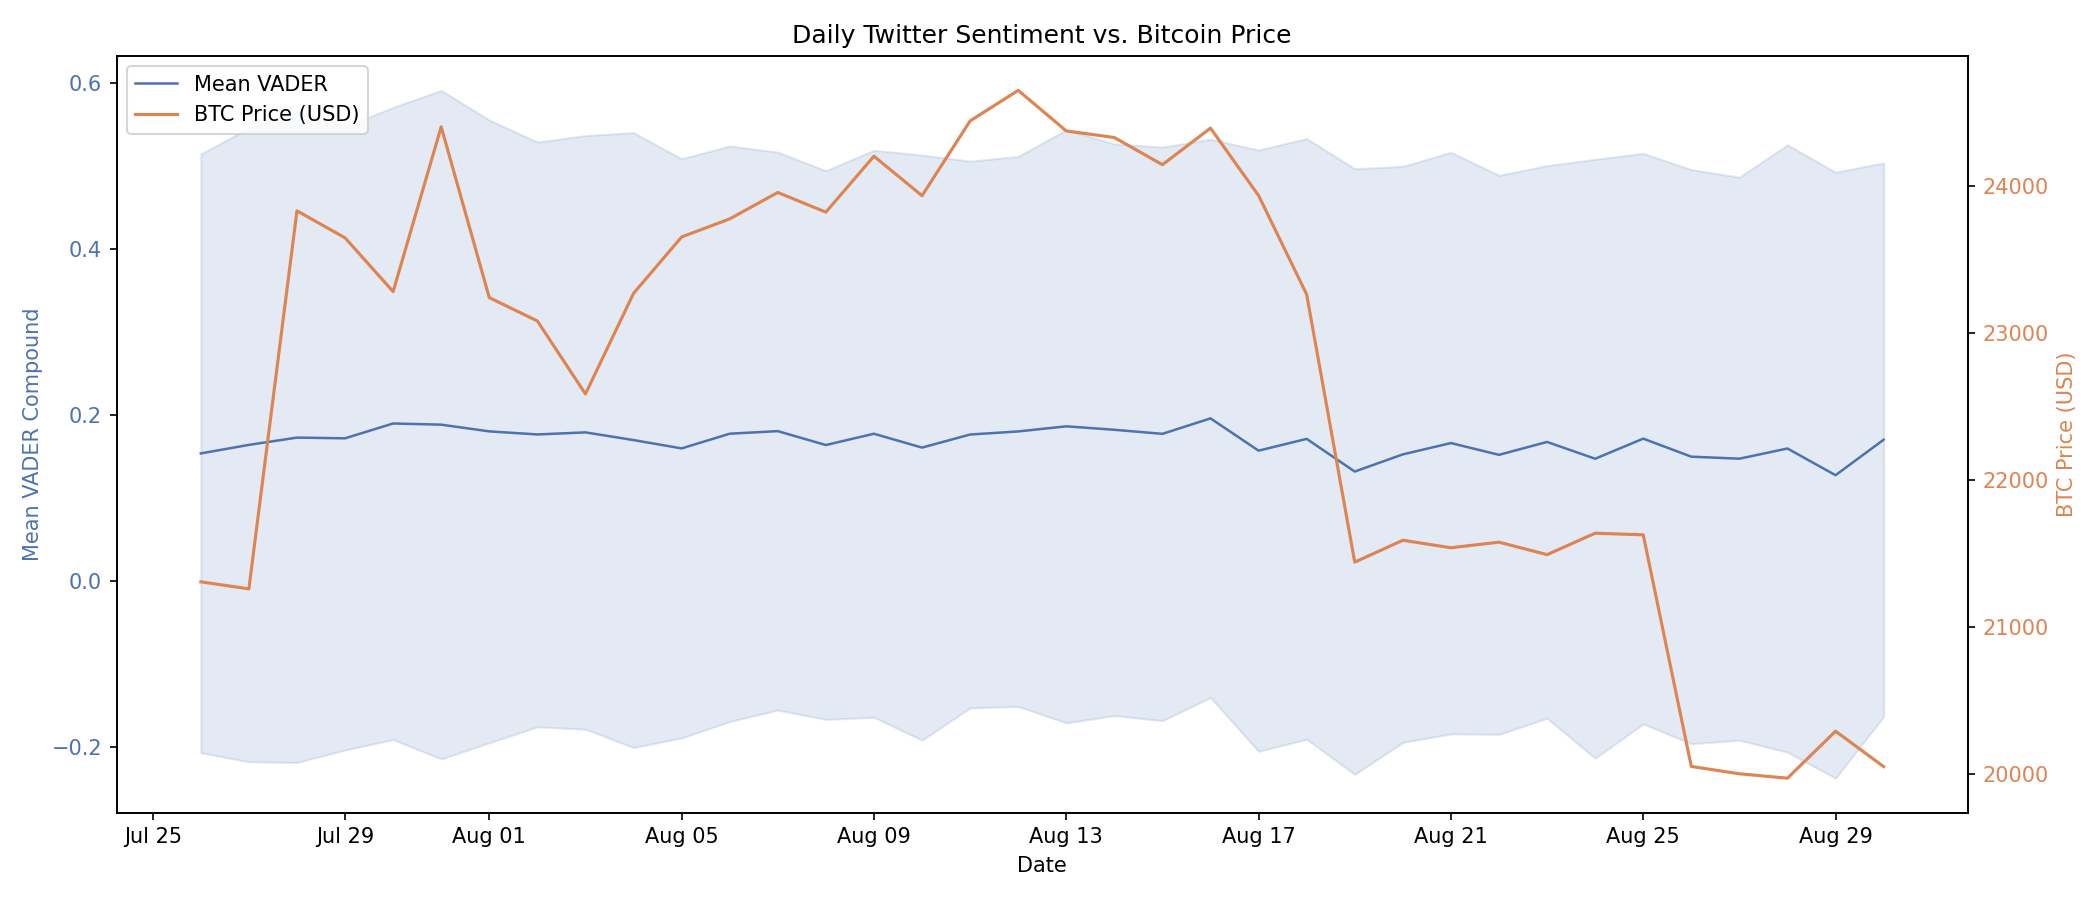
\includegraphics[width=0.95\textwidth]{../results/figures/sentiment_vs_price.png}
\caption{Дневная динамика средней тональности VADER (левая ось) и цены BTC/USD
(правая ось), июль--август 2022 г.}
\label{fig:sent_vs_price}
\end{figure}

\subsection{График 2: Лагированные корреляции}

\begin{figure}[H]
\centering
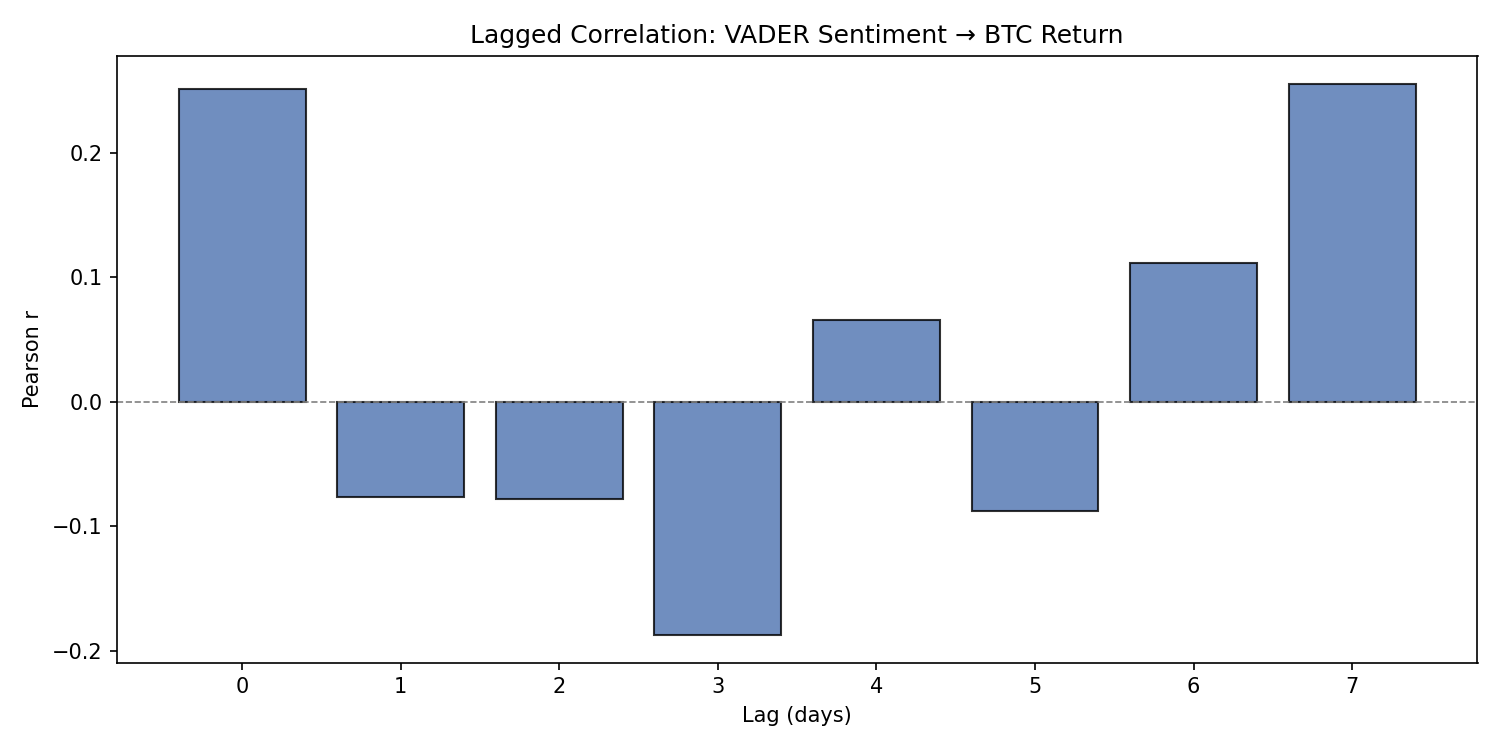
\includegraphics[width=0.85\textwidth]{../results/figures/lagged_correlation.png}
\caption{Корреляция Пирсона между VADER compound и доходностью BTC при лагах 0--7 дней.
Звёздочка (*) обозначает $p < 0.05$.}
\label{fig:lag_corr}
\end{figure}

\subsection{График 3: Корреляционная матрица}

\begin{figure}[H]
\centering
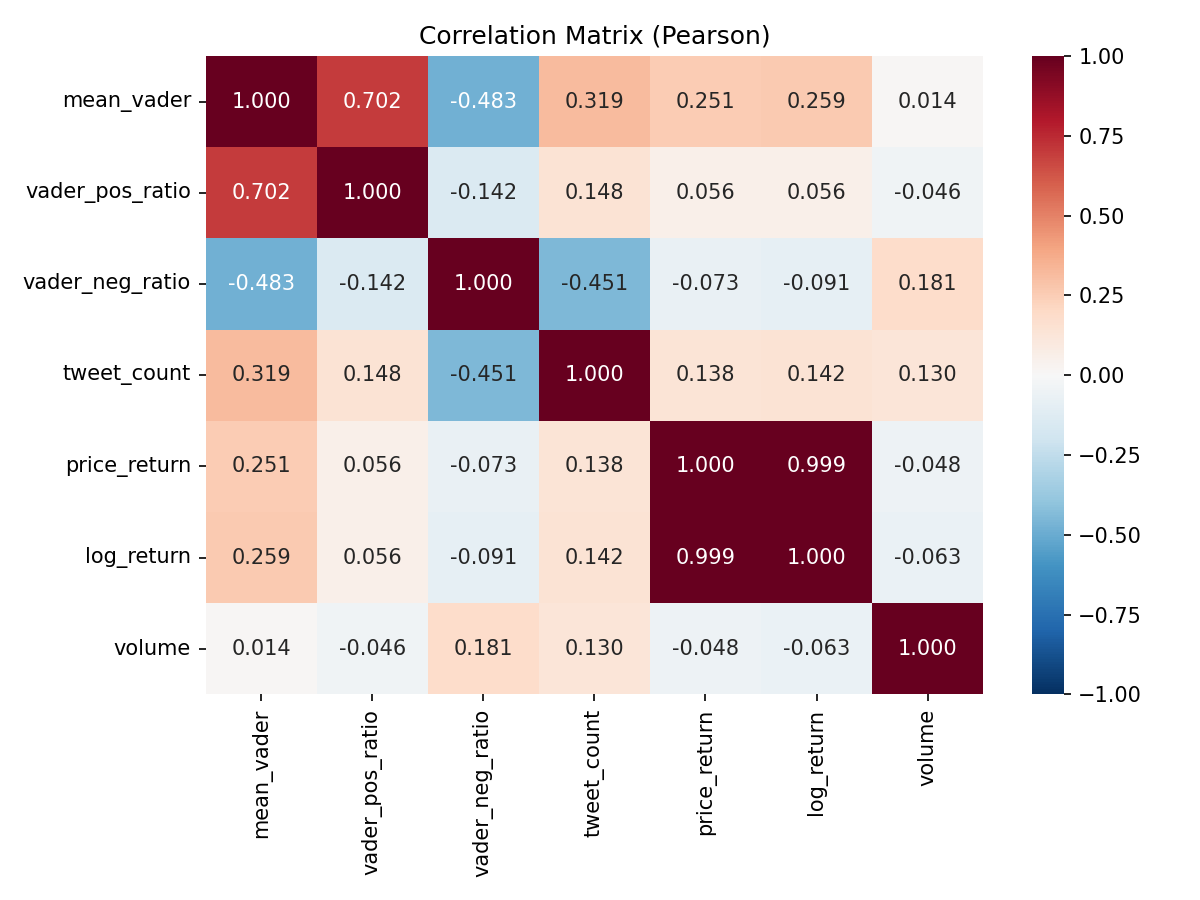
\includegraphics[width=0.8\textwidth]{../results/figures/correlation_heatmap.png}
\caption{Матрица корреляций Пирсона между ключевыми переменными.}
\label{fig:heatmap}
\end{figure}

\subsection{График 4: Распределение VADER compound}

\begin{figure}[H]
\centering
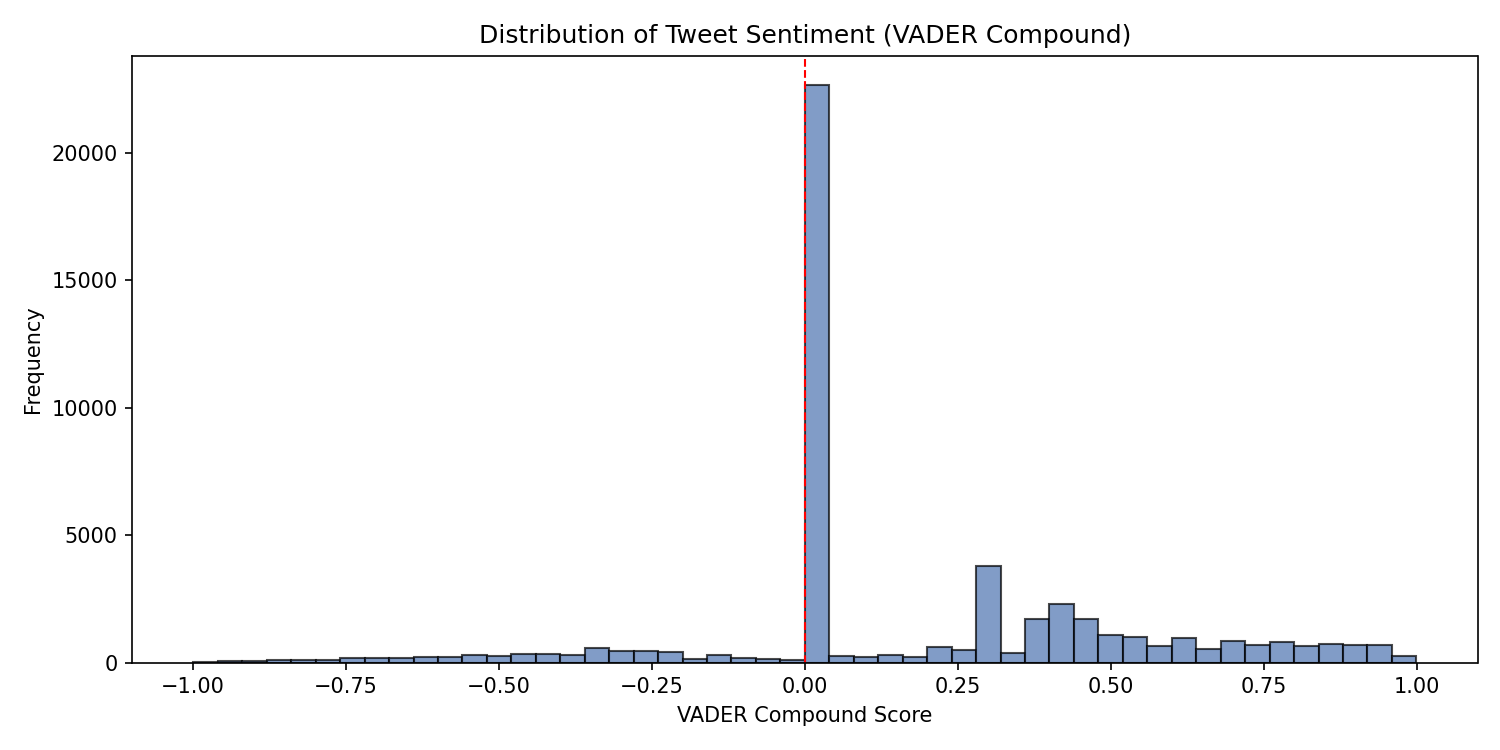
\includegraphics[width=0.85\textwidth]{../results/figures/sentiment_distribution.png}
\caption{Гистограмма распределения VADER compound score по всем твитам выборки.
Красная вертикальная линия --- нулевое значение.}
\label{fig:vader_dist}
\end{figure}

\subsection{График 5: Scatter --- тональность vs доходность}

\begin{figure}[H]
\centering
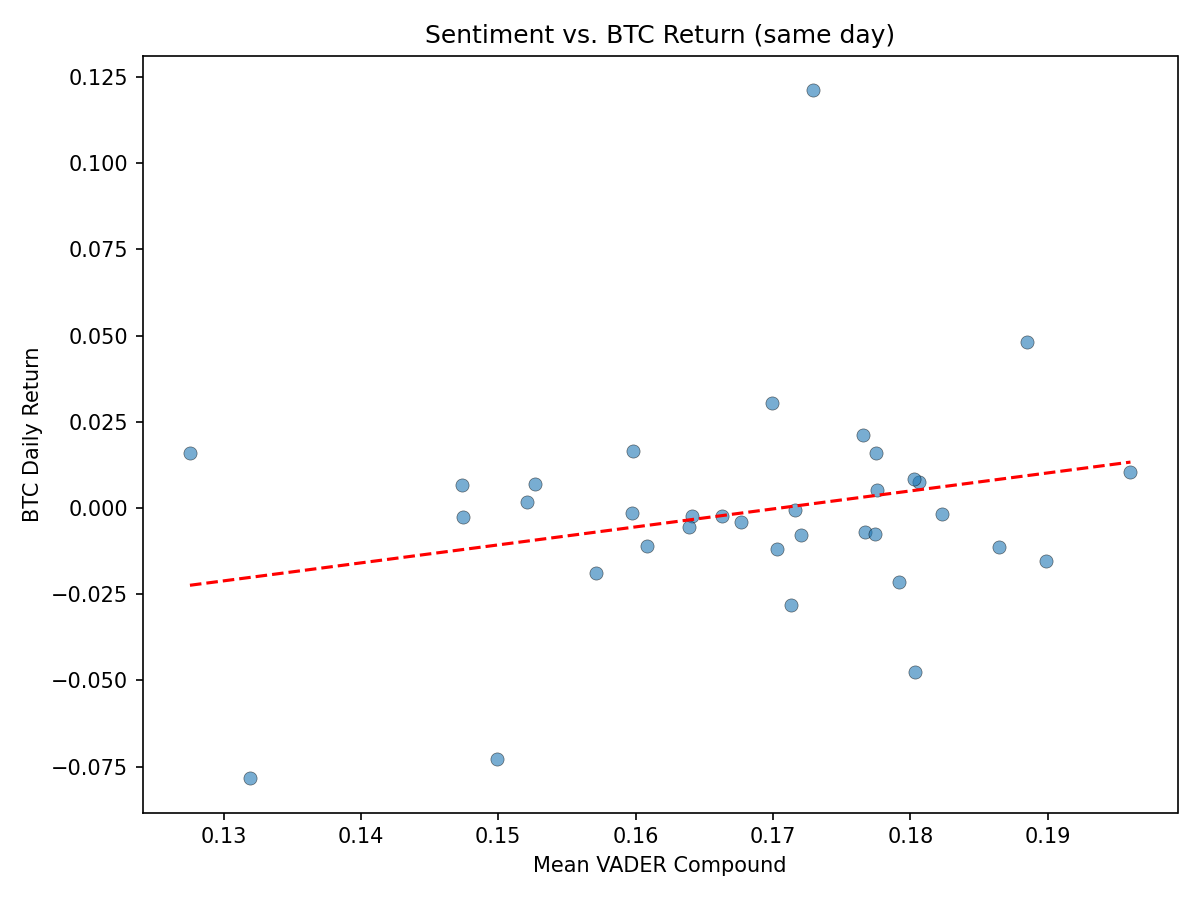
\includegraphics[width=0.8\textwidth]{../results/figures/scatter_sentiment_return.png}
\caption{Диаграмма рассеяния: дневное среднее VADER compound vs дневная доходность BTC.
Пунктирная линия --- линейная регрессия.}
\label{fig:scatter}
\end{figure}

\subsection{График 6: Объём твитов}

\begin{figure}[H]
\centering
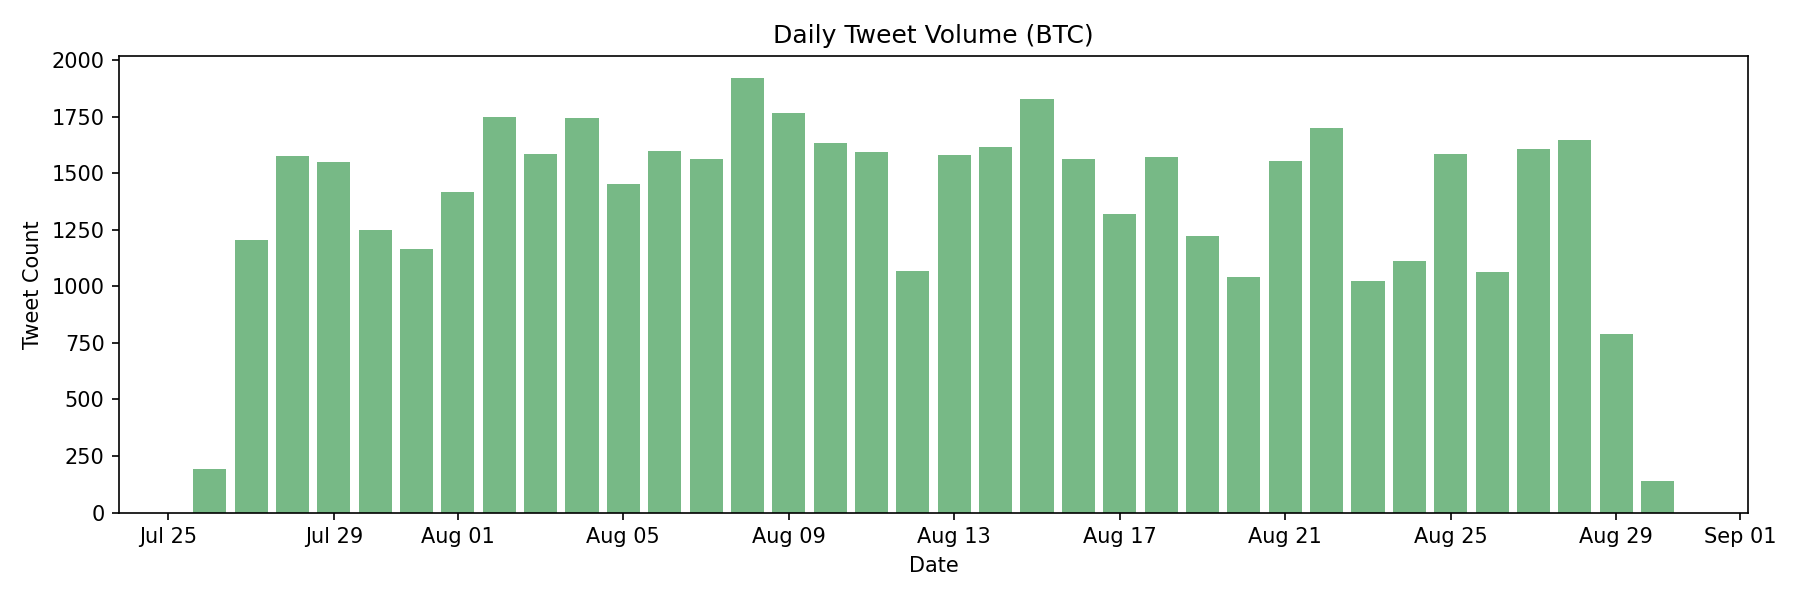
\includegraphics[width=0.9\textwidth]{../results/figures/tweet_volume.png}
\caption{Ежедневное число BTC-твитов в выборке.}
\label{fig:volume}
\end{figure}

\subsection{График 7: Сравнение VADER и FinBERT}

\begin{figure}[H]
\centering
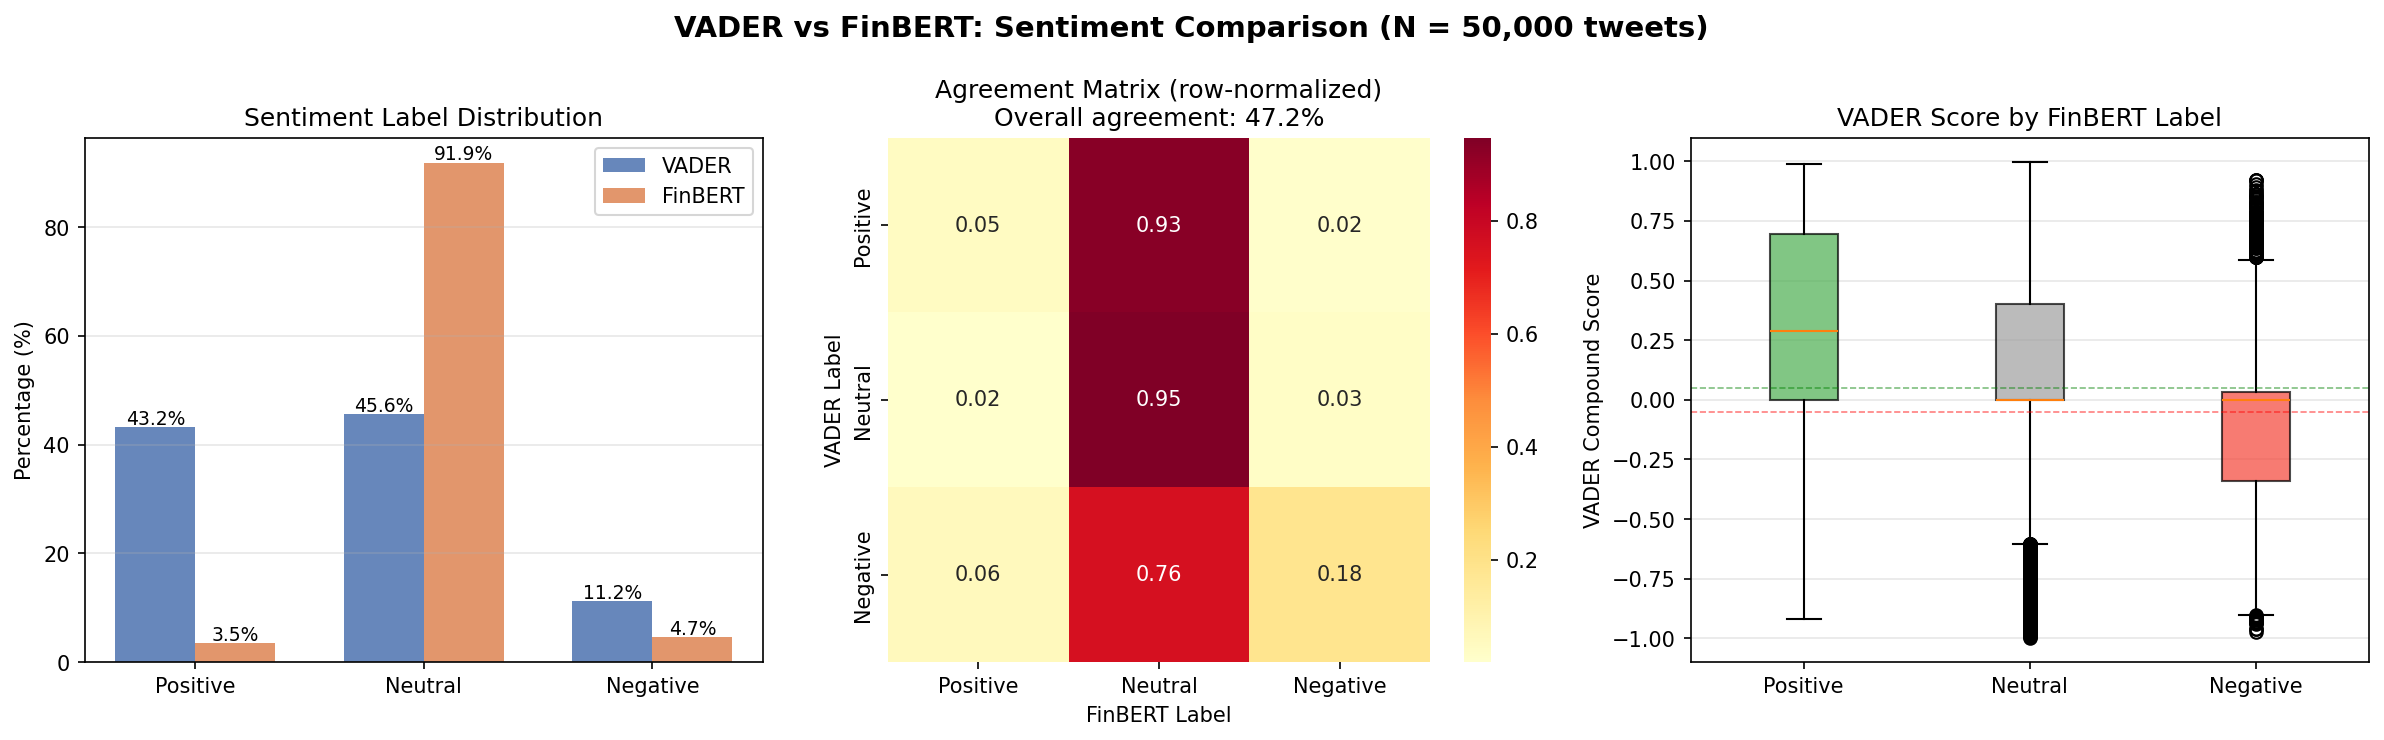
\includegraphics[width=0.95\textwidth]{../results/figures/vader_vs_finbert_comparison.png}
\caption{Сравнение методов анализа тональности: (a) распределение меток,
(b) нормализованная матрица согласия, (c) распределение VADER compound
по классам FinBERT.}
\label{fig:comparison}
\end{figure}

% ═══════════════════════════════════════════
% 4. АНАЛИЗ И ОБСУЖДЕНИЕ
% ═══════════════════════════════════════════

\section{Анализ и обсуждение результатов}

\subsection{Проверка гипотез}

\textbf{$H_1$ (корреляция):} \textit{Не подтверждена.}
Ни одна из лагированных корреляций не достигает уровня значимости $\alpha = 0.05$.
Наибольшее значение Pearson $r = 0.251$ (лаг 0, $p = 0.146$) указывает на слабую
положительную тенденцию, но объём данных (36 дней) недостаточен для
статистического подтверждения.

\textbf{$H_2$ (Грейнджер-каузальность):} \textit{Не подтверждена.}
Тест Грейнджера не выявил значимой предсказательной связи ни при одном лаге.
Это согласуется с гипотезой эффективного рынка (EMH) --- если информация
из Twitter уже инкорпорирована в цену, лагированная связь будет отсутствовать.

\textbf{$H_3$ (различие методов):} \textit{Подтверждена.}
Согласованность VADER и FinBERT составляет лишь 47.22\%, что свидетельствует
о принципиально различной интерпретации тональности криптовалютных текстов.

\subsection{Сравнение с baseline}

В качестве baseline выступает VADER --- метод, не требующий обучения.
FinBERT, несмотря на 109.5 млн параметров, демонстрирует значительно
менее дифференцированное распределение меток (91.89\% нейтральных).

Это позволяет предположить, что для неформальных крипто-текстов в Twitter
лексиконный подход (VADER) обеспечивает более информативное распределение,
тогда как FinBERT, обученный на формальных финансовых текстах,
может требовать дообучения (fine-tuning) на криптовалютном корпусе.

\subsection{Ограничения}

\begin{enumerate}
  \item \textbf{Короткий временной период:} 36 дней (июль--август 2022)
        ограничивает статистическую мощность тестов.
  \item \textbf{Одна криптовалюта:} анализировался только Bitcoin.
  \item \textbf{Без учёта объёма:} не учитывалось влияние торгового объёма
        и рыночной капитализации.
  \item \textbf{FinBERT без fine-tuning:} модель использовалась <<как есть>>,
        без дообучения на крипто-текстах.
\end{enumerate}

\subsection{Направления развития (ВКР)}

\begin{enumerate}
  \item Расширение датасета до полных 664\,918 твитов.
  \item Мультивалютный анализ (ETH, BNB).
  \item Fine-tuning FinBERT на криптовалютном корпусе.
  \item Использование моделей машинного обучения для прогнозирования цен.
  \item Разработка веб-интерфейса для real-time мониторинга тональности.
\end{enumerate}

% ═══════════════════════════════════════════
% 5. ВЕРИФИКАЦИЯ
% ═══════════════════════════════════════════

\section{Верификация}

Корректность системы подтверждена:

\begin{enumerate}
  \item \textbf{Модульные тесты:} 28 тестов (pytest), 100\% passed.
  \item \textbf{CI/CD:} GitHub Actions автоматически проверяет тесты
        на Python 3.10, 3.11, 3.12 при каждом push.
  \item \textbf{Линтинг:} flake8 --- 0 ошибок.
  \item \textbf{Воспроизводимость:} результаты воспроизводятся при запуске
        с \texttt{--sample 50000} (seed=42).
\end{enumerate}

Репозиторий: \url{https://github.com/iragoum/nlp-crypto-sentiment-pipeline}

\end{document}
